\section{Experimentation \& Results}\label{sec:results}


A number of computational experiments are conducted to highlight unique features
enabled by the DRE in Cyclus. Each experiment is performed by solving instances
of the DRE using both the \greedy heuristic and to optimality with the
branch-and-bound solver \cbc. A UOX-MOX one-pass recycle system with all
required fuel cycle facilities is taken as the \basecase scenario in order to
reduce the complexity of the fuel cycle and highlight departures from available
simulators. For simplicity of demonstration, reactors are assumed to refuel
completely with a single commodity rather than a combination of fuel types as is
done in practice. A simulation time frame of 50 years is chosen with one-month
time-steps (totaling 600 simulation time steps), sufficient to display all
relevant effects. The nominal parameters of all common facilities in the
simulation are shown in \cite{gidden_dre_2016}.

The \basecase scenario is not process constrained (i.e., it is constrained only
by the dynamics of Pu availability in the recycling stream). Reactors are
allowed to be fueled by either UOX or MOX, with a preference for MOX over UOX,
and refuel one-third of their total core mass every 18 months. Spent UOX fuel is
allowed to be recycled, whereas spent MOX fuel is sent directly to a
repository. In order to involve dynamism in the simulation, the population
reactors grows linearly over time at a rate of 1 reactor every 5 years. An
initial population of 20 reactors are deployed individually in each of the first
20 time-steps of the simulation as shown in Figure \ref{fig:deploy}. Note that
deployments are staggered in the initial period in order to avoid supply/demand
clustering effect. A diagram of the full \basecase fuel cycle is shown in Figure
\ref{fig:base}.

\begin{figure}
  \begin{center}
    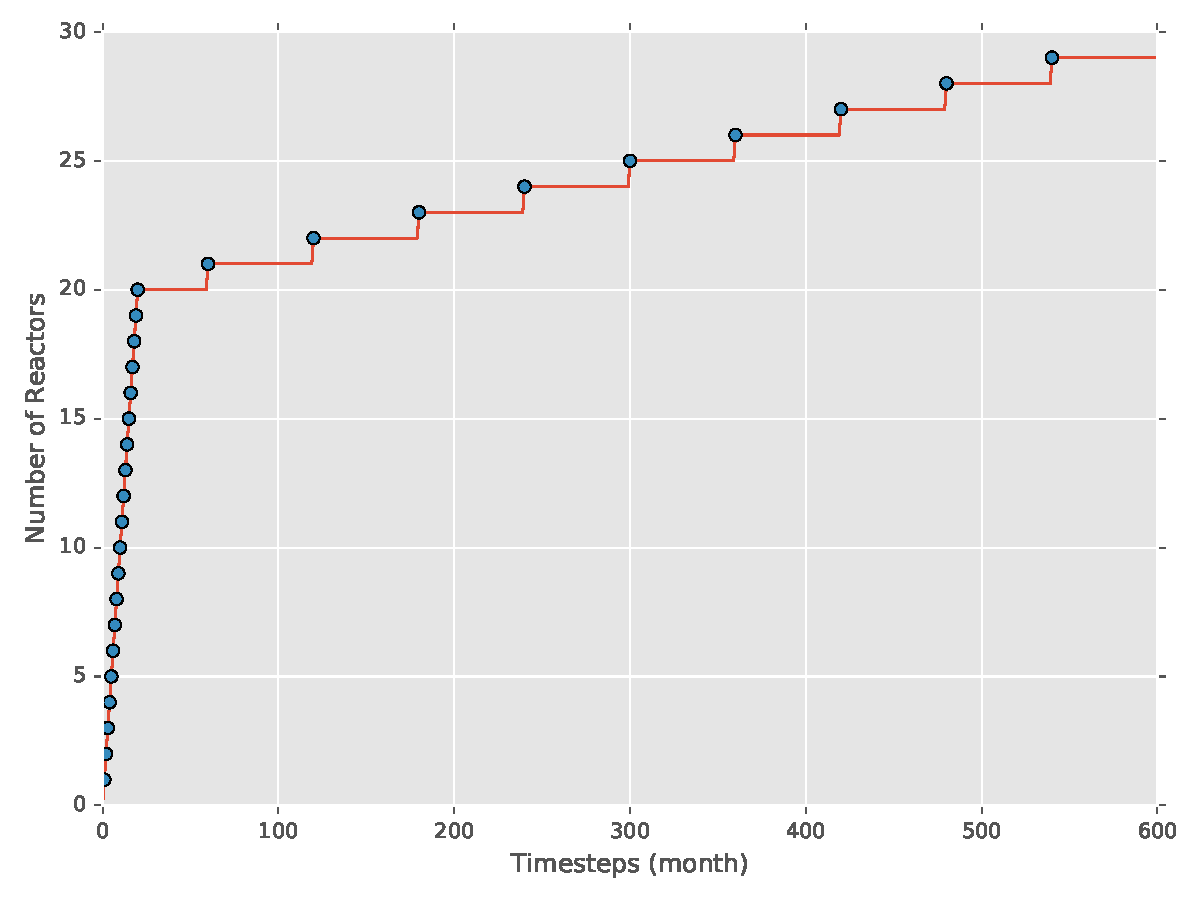
\includegraphics[width=\columnwidth]{rxtr_deploy.pdf}
    \caption[]{
      \label{fig:deploy}
      \reactor deployment in each simulation as a function of simulation time
      steps. Each point in the graph is a reactor being deployed in the
      simulation. Deployments for the \tariff scenario are distinguished by
      color: blue represents deployments in Region A and purple represents
      deployments in Region B.}
  \end{center}
\end{figure}

\begin{figure}
  \begin{center}
    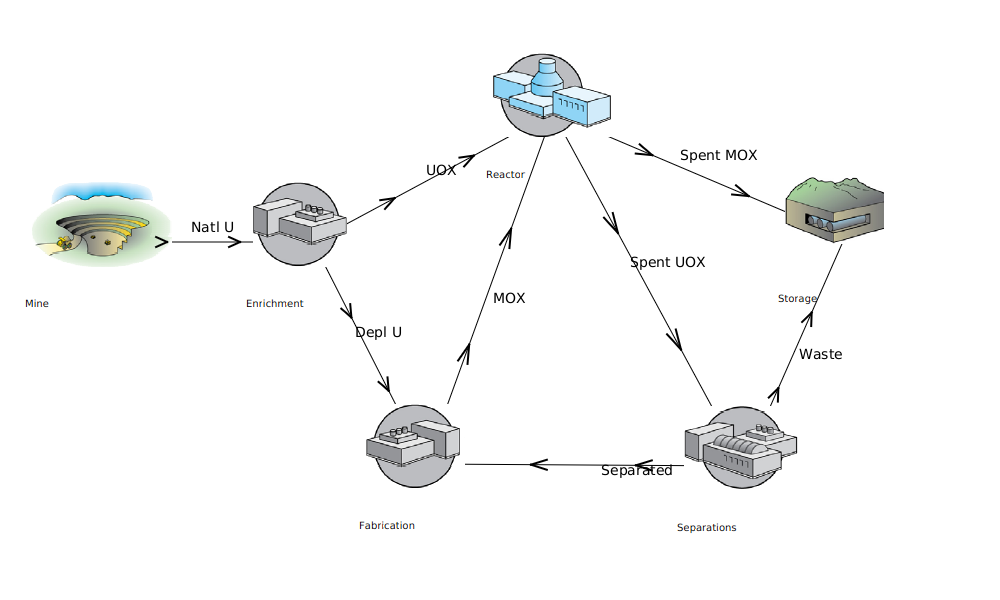
\includegraphics[width=\columnwidth]{base_case_fc}
    \caption[]{
      \label{fig:base}
      Material routing between in the \basecase scenario, single-pass MOX fuel
      cycle. Possible arc flows are labeled with commodity names.}
  \end{center}
\end{figure}

Three perturbations from the \basecase scenario are used to provide examples of
modeling capability enabled through the use of the DRE. The scenarios are
summarized in Table \ref{scenarios} below and described in more detail in the
following sections. 

\begin{table}[]
\centering
\caption{Short Descriptions of Scenarios Ran}
\label{scenarios}
\begin{tabularx}{\textwidth}{|p{1.5cm}|p{1.5cm}|X|X|}
\hline
\textbf{Scenario  Name} & \textbf{Scenario Handle} & \textbf{Primary Departure from Base Case}                & \textbf{Capability Highlighted}                             \\ \hline
Separations Outage      & \outage                   & Separations facility halts operation mid-simulation      & System flexibility to recycling facilities operation        \\ \hline
External MOX Supplier   & \external                 & An additional supplier of MOX enters mid-simulation      & System flexibility to entry and exit of commodity suppliers \\ \hline
Regional Tariffs        & \tariff                   & Two regions are modeled with dynamic trade relationships & Ability to model nontrivial international relationships     \\ \hline
\end{tabularx}
\end{table}

\subsection{Separations Outage: Fuel Cycles with Supply Disruption}

The DRE provides a unifying framework in which any instance of supply and demand
can be formulated and solved. This flexibility lends itself well to dynamic
simulation in which the state of actors in a simulation, by definition, can
change as the simulation progresses. In order to show case the types of
simulations that are enabled by this feature, a fuel cycle simulation is
constructed that has multiple types of reactor fuel input and a defined supply
disruption within the recycled-fuel supply chain.

The chosen disruption is an outage of the separations facility shown in Figure
\ref{fig:base}. The outage begins at $t_i = 250$, lasts 50 time steps, ending at
$t_f = 300$. During the outage, the remaining facilities in the supply chain
operate normally, and the flow of fuel into and out of reactors adapts according
to the state of available fresh fuel. Importantly, neither the \separations or
\fabrication facilities have throughput constraints, i.e., both facilities are
immediately able to process any quantity of fuel.

A comparison of the inventories of plutonium (Pu) in each facility type of
interest among the \basecase and \outage scenarios is shown in Figure
\ref{fig:outage}. As can be seen in Figure \ref{fig:baseinv-outage}, the
quantity of MOX in \reactors is under a dynamic equilibrium, oscillating between
the maximum quantity allowable in the system and one refueling quantity less
than the maximum, based on refueling schedules. The equilibrium value increases
in a stair-step-function manner as the number of reactors increases to being
able to provide sufficient used UOX for the next marginal refueling quantity of
MOX. The quantity of MOX in \fabrication oscillates between a minimal value and
a maximum value which is sufficient for a single reactor's refueling
quantity. As soon as there is sufficient MOX fuel for another refueling
\textit{and} a reactor makes a request to be refueled, it is provided the
quantity of MOX in of fresh fuel. Finally, \separations separates the various
actinides of used fuel and passes on fissile isotopes to \fabrication, thus
maintaining a small oscillating inventory in each timestep.

\begin{figure}
  \centering
  \begin{minipage}{0.67\textwidth}
    \centering 
    \subfloat[Pu inventories in the \basecase scenario.]{
      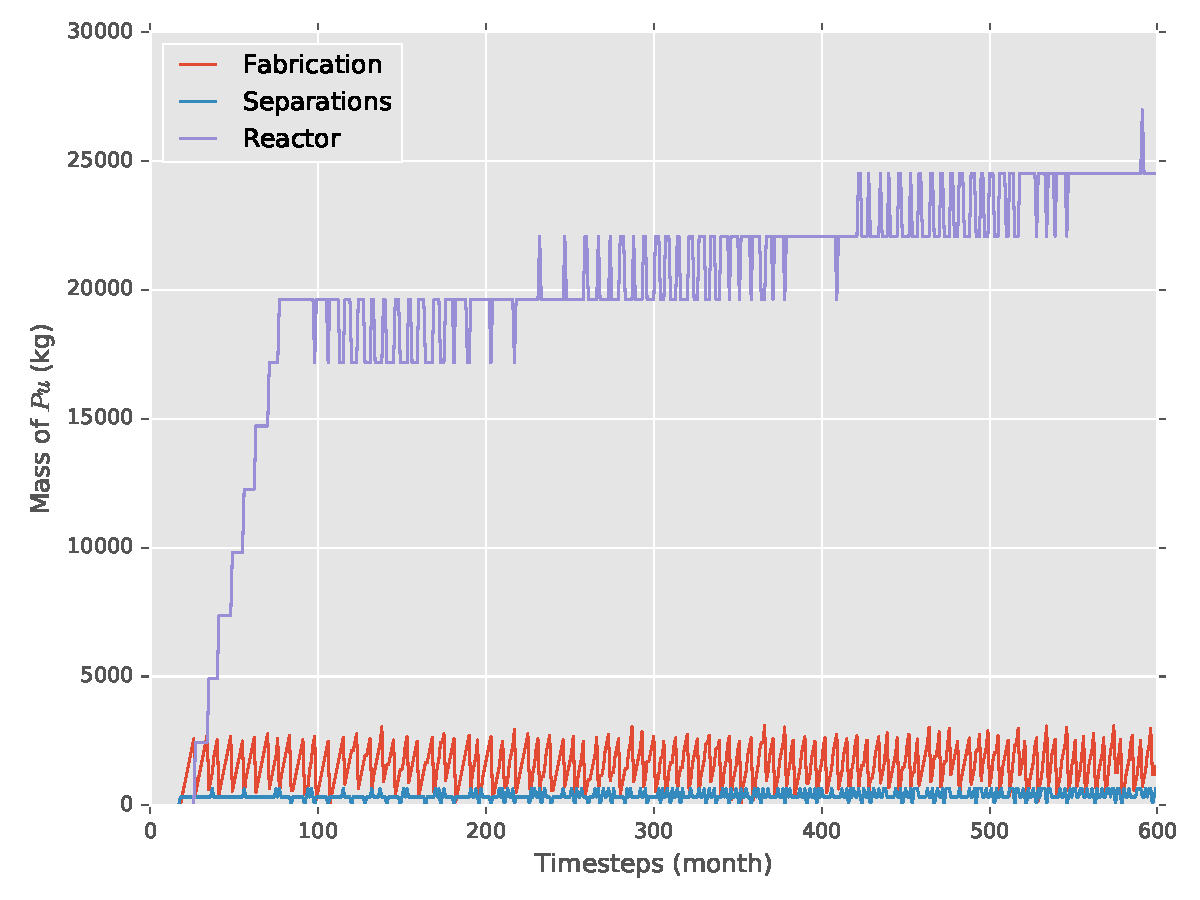
\includegraphics[height=0.3\textheight]{outage_invs_a.pdf}
      \label{fig:baseinv-outage}}
    \vfill 
    \subfloat[Pu inventories in the \outage scenario.]{
      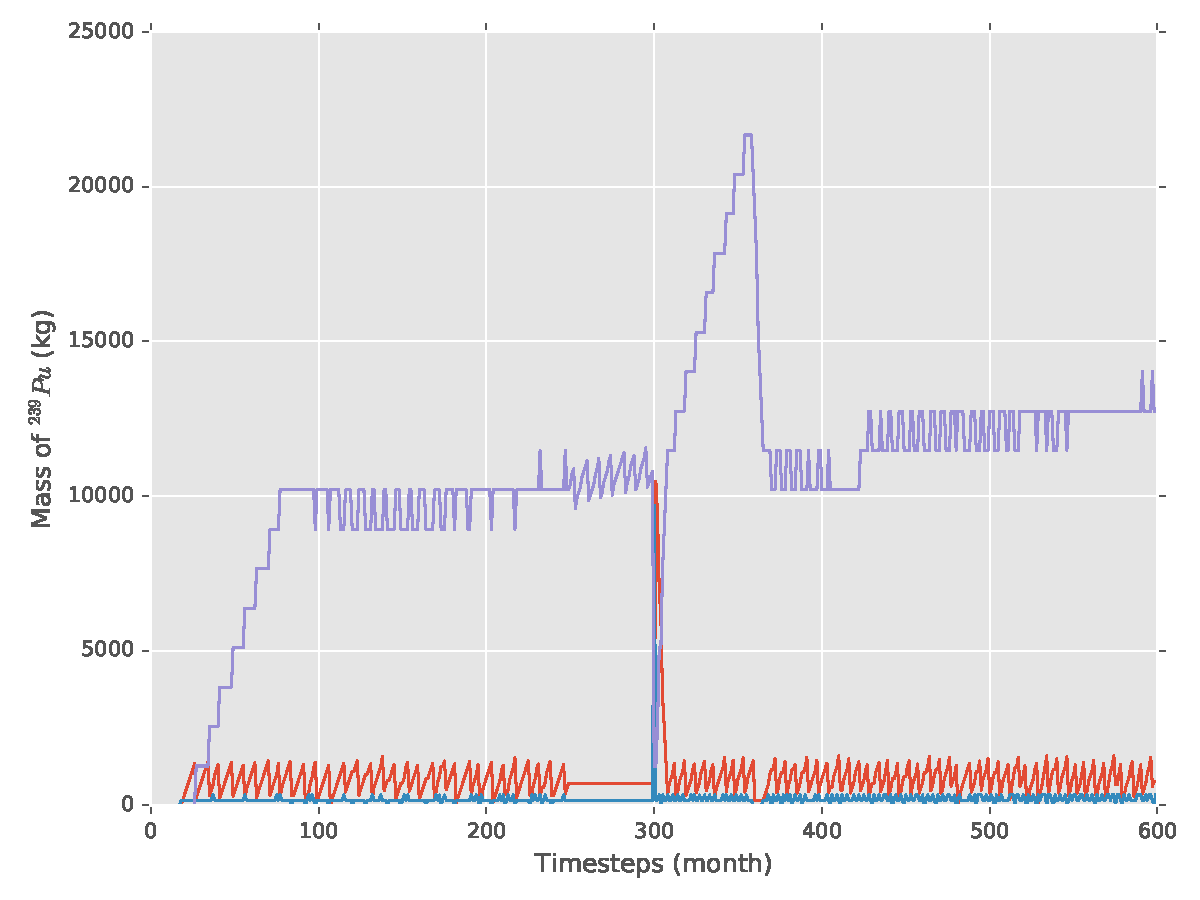
\includegraphics[height=0.3\textheight]{outage_invs_b.pdf}
    \label{fig:outageinv}}
  \end{minipage}%
  \begin{minipage}{0.33\textwidth}
    \centering
    \subfloat[A close-up of the \outage scenario perturbation.]{
      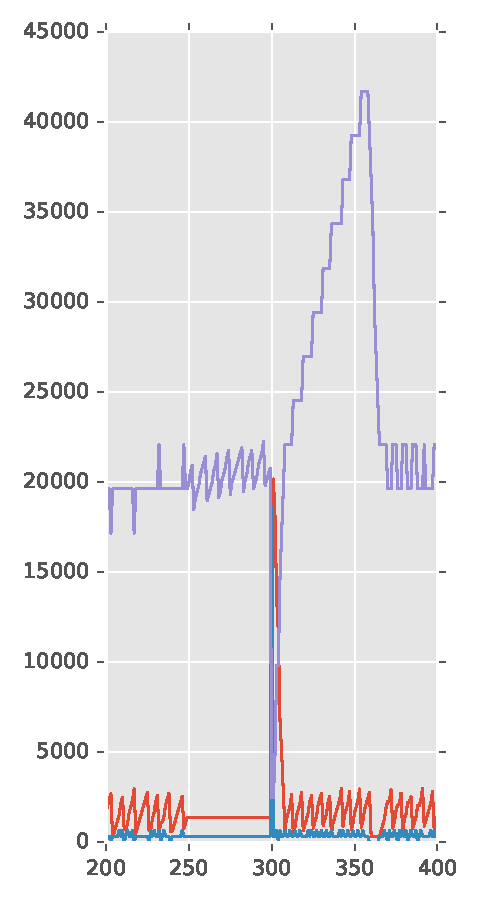
\includegraphics[height=0.6\textheight]{outage_invs_c.pdf}
      \label{fig:outagezoom}}
  \end{minipage}%
  \caption[]{
    \label{fig:outage}
    Facility inventories of Pu in \basecase and \outage scenarios.}
\end{figure}

The dynamic equilibrium behavior changes in the \outage scenario after the
initial outage time, $t_i$, as is observable in Figures \ref{fig:outageinv} and
\ref{fig:outagezoom}. Because the outage occurs in \separations, which takes
input from the \reactors and provides output to \fabrication, the inventories of
both \separations and \fabrication remain constant for the duration of the
outage period. The inventory of Pu in \reactors continues to oscillate
because MOX assemblies are discharged and continue to be sent to \storage,
whereas spent UOX assemblies (with significant Pu inventories) are stored on
site. In the first timestep of renewed service of \separations, $t_f$, the
entirety of the pent-up store of used fuel in \reactors is send to \separations,
reducing the inventory to zero, causing the delta-function behavior in \reactor
flows seen in Figure \ref{fig:outagezoom} at $t = t_f$. \separations then
extracts all of Pu in a single timestep, sending it to \fabrication and
causing the delta-function behavior in \separations flows seen in Figure
\ref{fig:outagezoom} at $t = t_f + 1$. Finally, the stock of Pu in \reactors
after the outage increases due to the higher availability of MOX fuel in
\fabrication, until the dynamic equilibrium returns. The length of the
perturbation is function of both the amount of Pu required per refueling and
the number of refuelings that occurs during the outage. The more refuelings that
happen during the outage, the more excess MOX assemblies can be made, thus
continuing the dynamic equilibrium perturbation.

\subsection{External MOX Supplier: Fuel Cycles with Demand Fungibility}

The DRE allows for both positive and negative perturbations in fuel
availability. While the \outage scenario models a case where there is a
supply-chain disruption, the \external scenario models a case where there is an
injection of a preferred commodity source. An example of such a scenario
occurring in the real world includes the down-blending of military-grade fuel
sources, such as the MOX Fuel Fabrication Facility, in which a preferred fuel
commodity is introduced, and the Megatons to Megawatts (MT2MW) program, where a
preferred fuel fabrication commodity is introduced at the enrichment-fabrication
facility interface.

In the \external scenario, an external source of MOX fuel enters halfway
through the simulation at $t = 250$, creating the fuel cycle shown in Figure
\ref{fig:military_fc}. The total quantity of fuel the external source can provide is
limited to 10 refueling quantities (where reactors refuel one third of their
total core mass in each cycle). Preferences are assigned such that reactors
prefer MOX from its normal cycle over MOX from the external source, i.e.,
$p_{\text{MOX}} > p_{\text{MOX, external}} > p_{\text{UOX}}$. Reactors request each
of the commodities, and thus the first 10 reactors to refuel after the external
source enters the simulation when no original MOX is available will be provided
with MOX from the external facility. Reactors will continue to request fuel from the
external facility for the remainder of the simulation, but will not receive any due
to the limited total inventory. This injection of a new fuel source also serves to
perturb the supply chain by delaying the amount of spent UOX available for
recycling.

\begin{figure}
  \begin{center}
    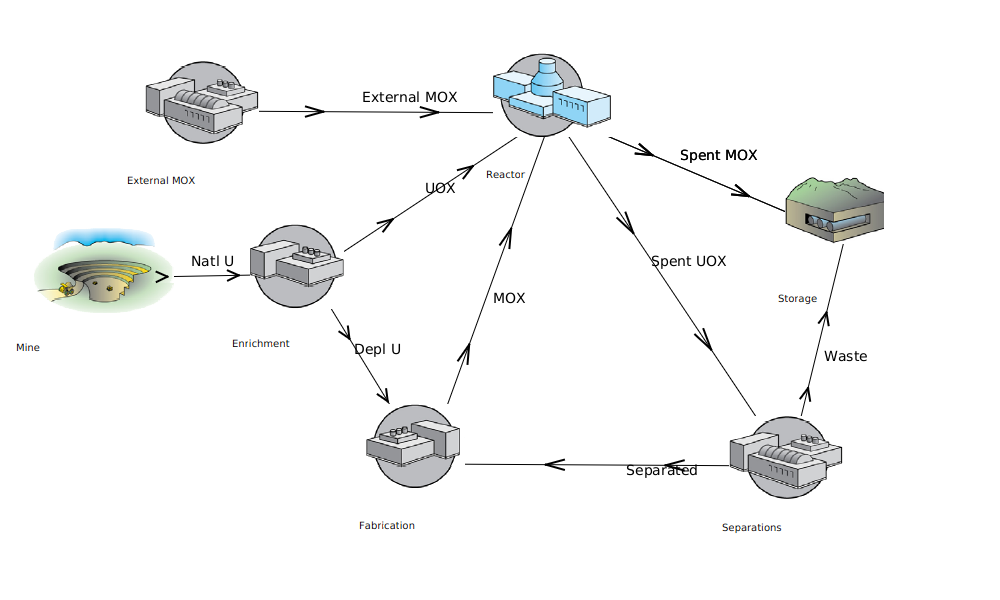
\includegraphics[width=\columnwidth]{external_fc}
    \caption[]{
      \label{fig:military_fc}
      Material routing between in the \external scenario fuel
      cycle. Possible arc flows are labeled with commodity names.}
  \end{center}
\end{figure}

The dynamic equilibrium of Pu inventories again changes with the \external
perturbation, as shown in Figure \ref{fig:military}. A number of new features
arise, however. First, the equilibrium value during the initial transient
increases by the total quantity of refueling quantities available from the
external source of MOX (in this case 10 refueling quantities). Second, the
equilibrium value upon exiting the transient is lower than the value upon its
entrance. This is due to the fact that the amount of spent UOX in the overall
recycle system has decreased, due to the usage of external MOX, thus reducing
the availability of MOX. The system has been shocked into a new dynamic
equilibrium, with Pu values slightly lower than the previous
equilibrium. This suggests that the injection of external recycled fuel can
reduce the level of which a system can sustain a recycling fuel cycle. Finally,
a small lag can be seen in the inventory of Pu in \fabrication, which is due
to a loss of available spent UOX due to the increased presence of spent MOX
exiting reactors that were able to utilize external MOX. The Pu inventories 
recover quickly from this transient, however.

\begin{figure}
  \centering
  \begin{minipage}{0.67\textwidth}
    \centering 
    \subfloat[Pu inventories in the \basecase scenario.]{
      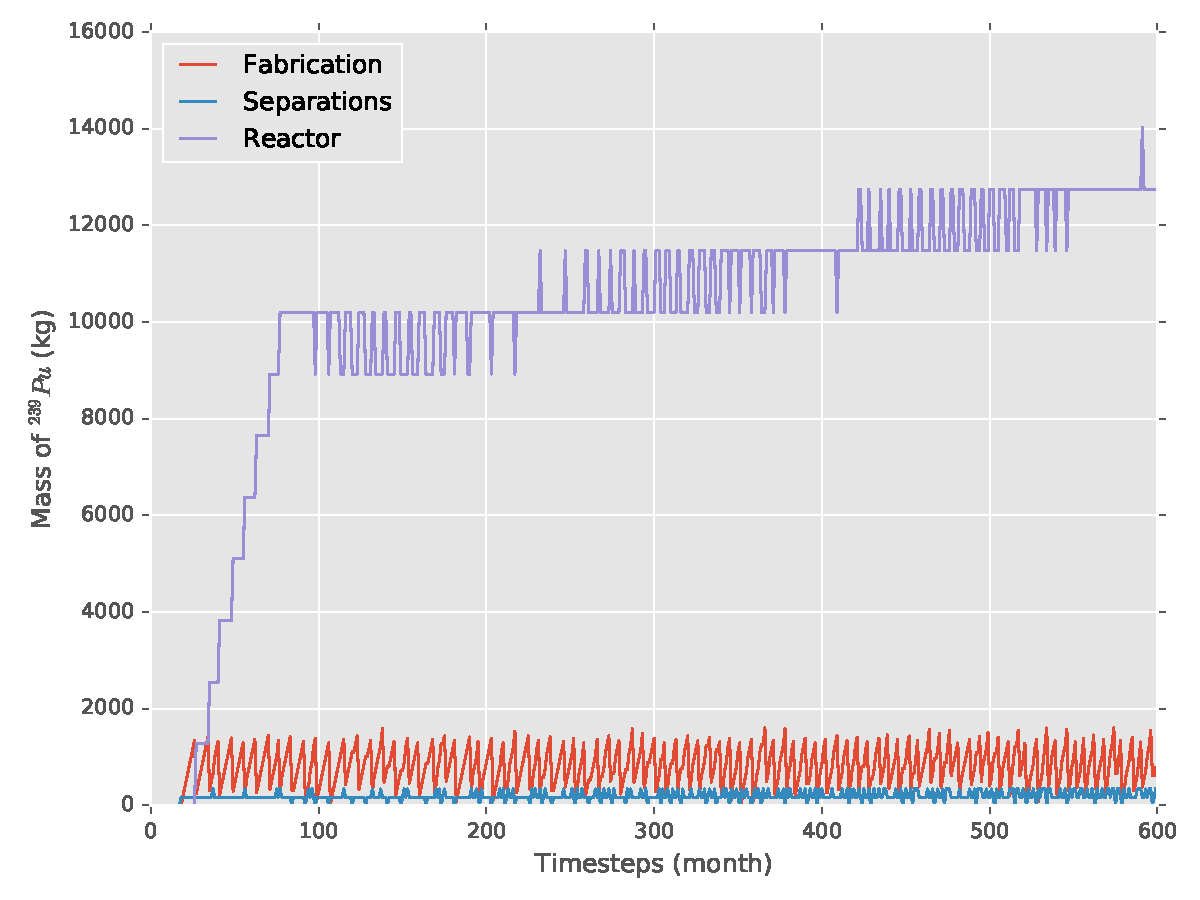
\includegraphics[height=0.3\textheight]{military_invs_a.pdf}
      \label{fig:baseinv-military}}
    \vfill 
    \subfloat[Pu inventories in the \external scenario.]{
      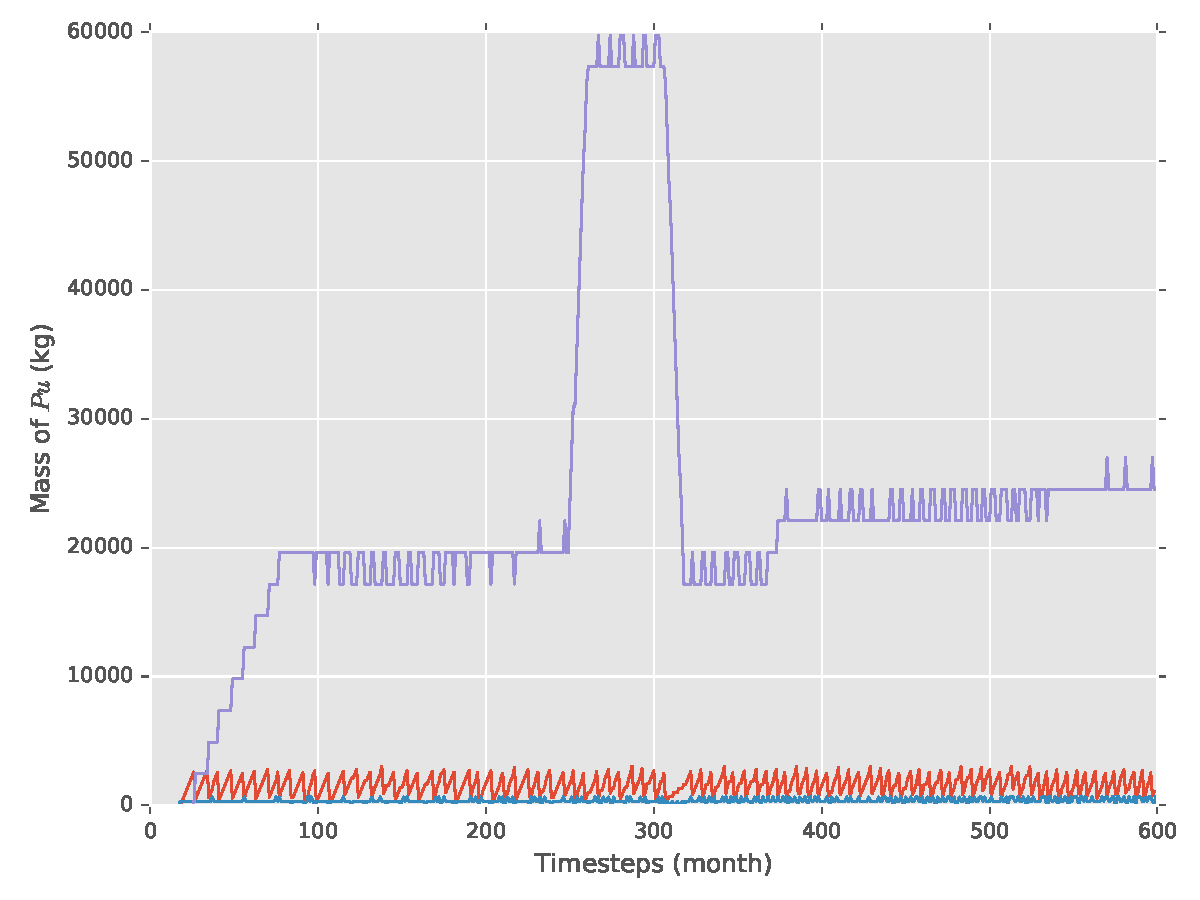
\includegraphics[height=0.3\textheight]{military_invs_b.pdf}
    \label{fig:militaryinv}}
  \end{minipage}%
  \begin{minipage}{0.33\textwidth}
    \centering
    \subfloat[A close-up of the \external scenario perturbation.]{
      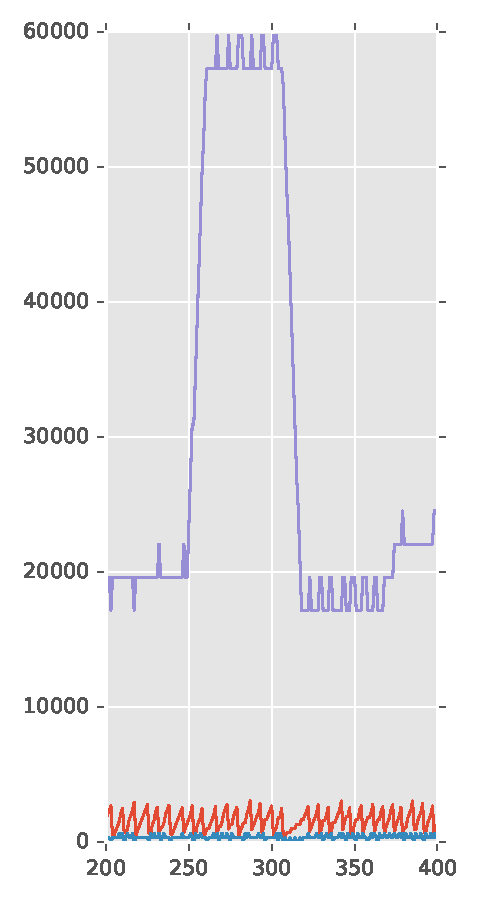
\includegraphics[height=0.6\textheight]{military_invs_c.pdf}
      \label{fig:militaryzoom}}
  \end{minipage}%
  \caption[]{
    \label{fig:military}
    Facility inventories of Pu in \basecase and \external scenarios.}
\end{figure}

\subsection{Regional Tariffs: Fuel Cycles with International Instruments}

One of the novel features of the DRE is the ability for different geographical
and managing entity representations to be laid over otherwise regional-agnostic
fuel cycles and affect the outcome of possible trades between those fuel
cycles. The \tariff two-region scenario showcases the ability to model
such situations.

Two regions, Region A and Region B, are modeled. Region A houses a fuel cycle
with both UOX and MOX-based fuel services, as in the \basecase scenario. The
same total number of \reactors are modeled in the scenario. Region A begins with
15 \reactors and Region B begins with 5 reactors. All reactor deployment as
shown in Figure \ref{fig:deploy} occurs in Region A.

In this scenario, Region A can provide UOX and MOX fuel services to other
regions using a fuel take-back model (all fuel provided as a service is returned
after it has been used in a reactor). Repatriation of fission products to the
lessee region is not modeled in this scenario for purposes of clarity. Region B
contains a simple, once-through fuel cycle. Although the scenario is somewhat
contrived in order to highlight a multi-commodity system under dynamic
behavioral change, such fuel service arrangements are present today in countries
that provide fuel for once-through fuel cycles, e.g., Russia
\cite{wnarussia2016}. The possible flow of commodities between fuel cycles is
shown in Figure \ref{fig:region}.

\begin{figure}
  \begin{center}
    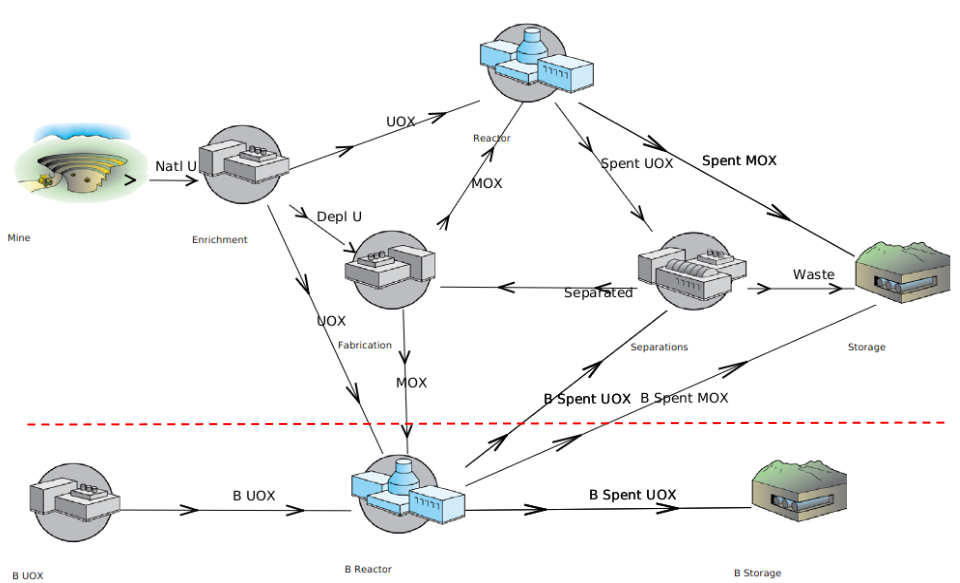
\includegraphics[width=\columnwidth]{tariff_fc_line}
    \caption[]{
      \label{fig:region}
      A two-region set of fuel cycles separated by a dotted-red line. The upper
      region (Region A) includes a one-pass MOX fuel cycle, and the bottom
      region (Region B) includes a once-through fuel cycle connected to the
      one-pass MOX fuel cycle. Note that all spent fuel that originated in
      Region A is returned to Region A's fuel cycle.}
  \end{center}
\end{figure}

Initially, preferences are set such that fuel trade from Region A to
Region B is preferred over Region B's domestic fuel production. In other words, a
preference distribution for fuel supplied to Region B has the following
relation

\begin{equation}\label{eqn:bigdefault}
  p_{MOX, a} > p_{UOX, a} > p_{UOX, b} > 1.
\end{equation}

\noindent
This preference distribution implies that Region B's domestic fuel cycle will
never be utilized -- it will always be fueled by Region A, as long as Region A
has available capacity. 

At some time $t_0$, a time-varying tariff is applied by Region B which perturbs
preference values along arcs connecting Region A fuel suppliers with Region B
fuel consumers. Consider a tariff defined by function in Equation
\ref{eqn:tariff} with preferences adhering to the relation provided in Equation
\ref{eqn:bigp1}, which guarantees a strict preference ordering under $f(t)$.

\begin{equation}\label{eqn:tariff}
f(t)
\begin{cases}
1, & \text{if } t < t_0 \\
\frac{p_{UOX, b} - 1}{p_{UOX, a}}, & \text{if } t_0 \leq t < t_1 \\
\frac{p_{UOX, b} - 1}{p_{MOX, a}}, & \text{if } t_1 \leq t < t_2
\end{cases} 
\end{equation}

\begin{equation}\label{eqn:bigp1}
  p_{UOX, b} \left( 1 - \frac{p_{UOX, a}}{p_{MOX, a}} \right) > 1.
\end{equation}

Choosing nominal values that satisfy Equations \ref{eqn:bigdefault} and
\ref{eqn:bigp1}, e.g., $p_{MOX, a} = 9$, $p_{UOX, a} = 4$, and $p_{UOX, b} = 2$,
one arrives at actual preference values as shown in Figure \ref{fig:prefs}. In
the \tariff scenario, $t_0$ is chosen to be 150 and $t_1$ is set to 300. The DRE
naturally handles the flow of commodities between \texttt{Facility} agents in
each \texttt{Region}, allowing the application of tariffs by the \texttt{Region}
agents.

\begin{figure}
  \begin{center}
    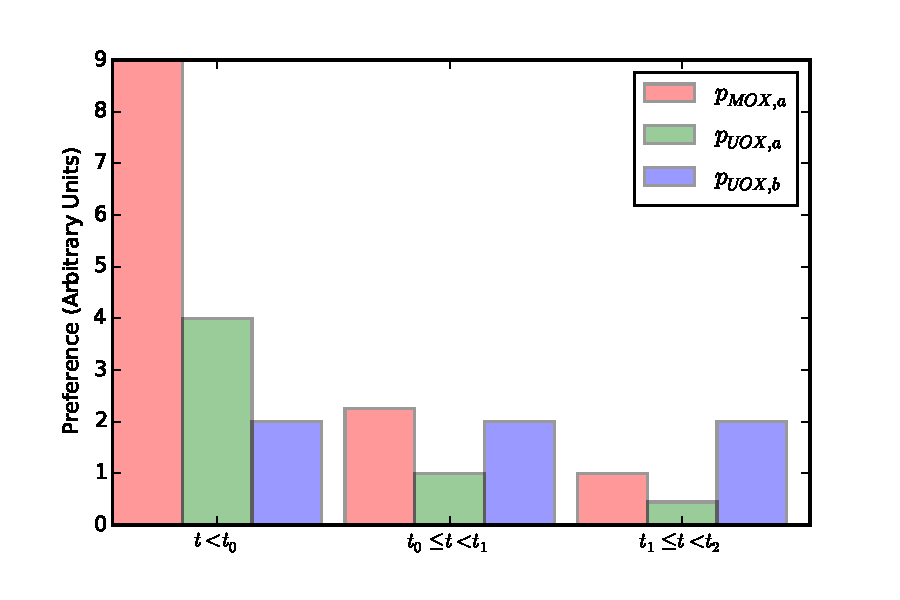
\includegraphics[width=\columnwidth]{tariff_prefs.pdf}
    \caption[]{
      \label{fig:prefs}
      Preference values for reactors in Region B for available fuel commodities
      in Region B as a function of time.}
  \end{center}
\end{figure}

The effects of time-dependent tariff application on the simulation can be seen
in Figure \ref{fig:tariff}. The front-end of Region B's fuel cycle is not
utilized until $t > t_0$; all fuel is provided from Region A. After $t_0$, the
majority of the fuel services required by \reactors in Region B comes from
Region B's own front end. However, it is still able to utilize the MOX-based
fuel services from Region A. Finally, after the final tariff is applied at
$t_1$, Region B's \reactors stop utilizing Region A's fuel cycle entirely.    

\begin{figure}
  \begin{center}
    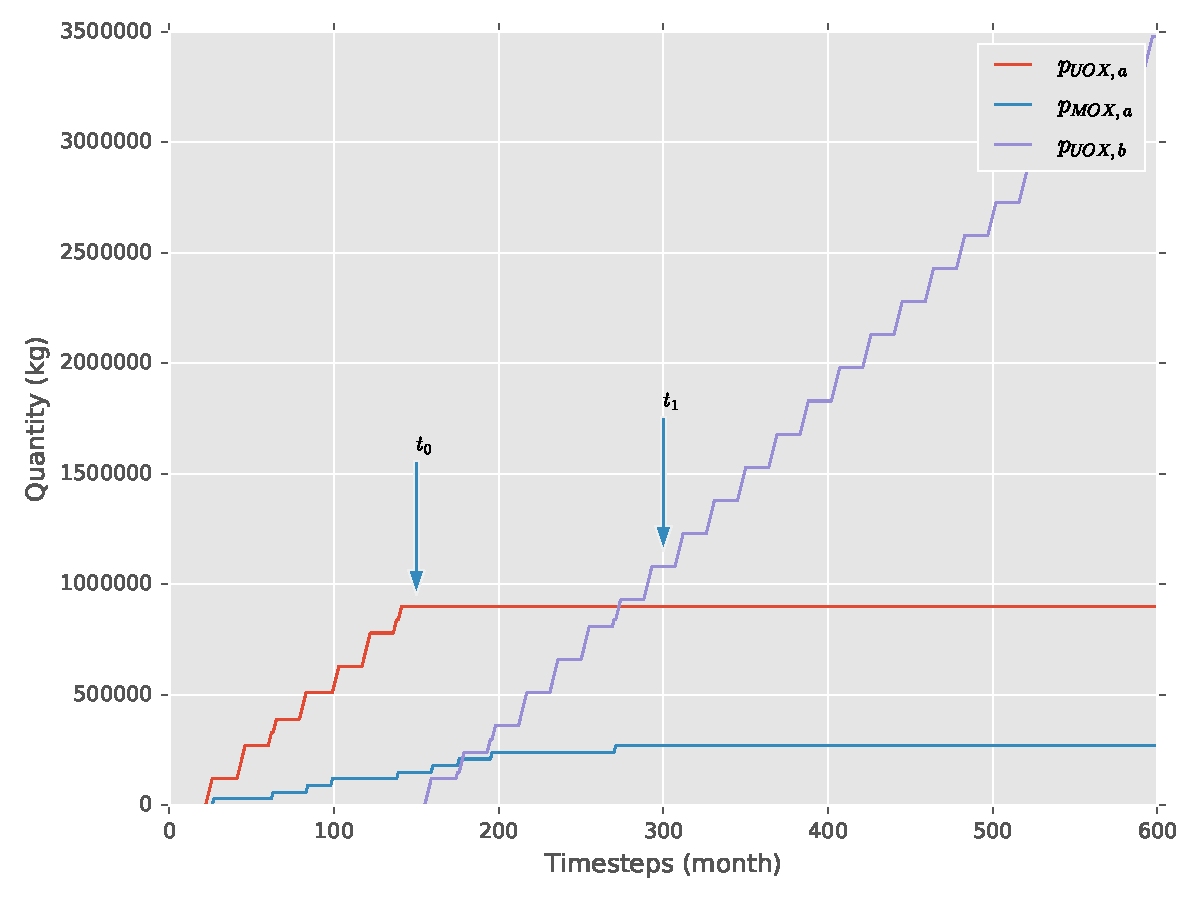
\includegraphics[width=\columnwidth]{tariff_b_reactor_flow.pdf}
    \caption[]{
      \label{fig:tariff}
      Cumulative flow of fuel into \reactors in Region B.}
  \end{center}
\end{figure}

\subsection{Comparisons between Scenarios}

In each scenario, the total amount of electricity generated is identical in
order to compare the mechanics and results of fuel supply and demand. Therefore,
comparisons between all scenarios is most easily made by observing the total
fuel usage by reactors for each commodity type. A summary of this metric is
provided in Figure \ref{fig:flows}. Figure \ref{fig:uoxflow} displays the
cumulative flow of UOX fuel into reactors over all scenarios which shows a
number of interesting effects. First, the \external scenario has the lowest
cumulative flow, which is expected of a scenario in which an external source of
non-UOX is provided.  The \outage scenario initially deviates from the \basecase
scenario, but eventually returns to match its cumulative UOX usage. This is due
to the fact that in the defined system, outages simply serve to store fuel. When
sufficient time has past after the outage, the system returns to its dynamic
equilibrium. Finally, the \tariff scenario utilizes the most UOX fuel of all,
providing an interesting case study of the effects of dynamic equilibrium. In
the \tariff scenario, there is a population of reactors that prefers UOX fuel
that is not sent to \separations (i.e., the UOX fuel in its own Region) over all
other sources in the simulation. Therefore, the population of Pu is reduced,
which reduces both the quantity and frequency of MOX availability. This, in
turn, increases overall UOX consumption. In short, MOX availability decreases
due to upstream supply chain effects, causing an increase in overall UOX
consumption.

Figure \ref{fig:moxflow} showcases the cumulative flow of MOX fuel into all
reactors as a function of simulation time step. Because reactors can be fueled
only with UOX or MOX, it represents the inverse of Figure \ref{fig:uoxflow}. For
example, whereas the \tariff scenario utilizes the most UOX, it utilizes the
least MOX for the same reasons. A number of additional features can be observed
in Figure \ref{fig:moxflow} dealing with departures from dynamic equilibrium of
the \basecase scenario. The undershooting and then overshooting of MOX
consumption in the \outage scenario is visible. During the outage, less MOX is
consumed, but immediately after the outage, excess MOX is consumed until there
is a return to dynamic equilibrium. Additionally, a reduction in the total
amount of MOX (sourced from recycled UOX) consumed is observed in the \external
scenario. This is due to a reduction in the available recycled UOX supply during
periods of external MOX consumption. In short, for each reload of external MOX,
the system loses a future amount of recyclable UOX.

\begin{figure}
  \centering
  \begin{minipage}{0.9\textwidth}
    \centering
    \subfloat[UOX flow.]{
      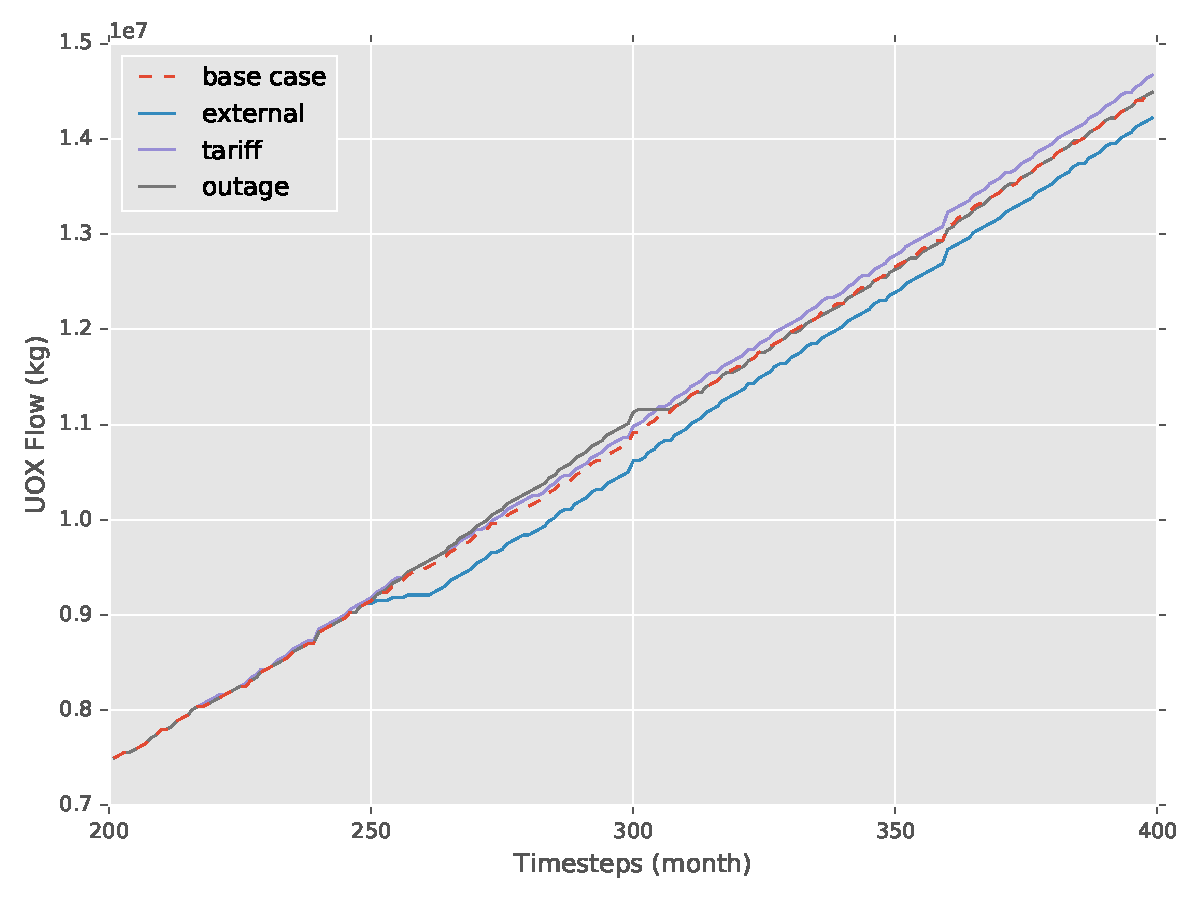
\includegraphics[width=0.9\textwidth]{uox_flow.pdf}\label{fig:uoxflow}}
    \vfill
    \subfloat[MOX flow]{
      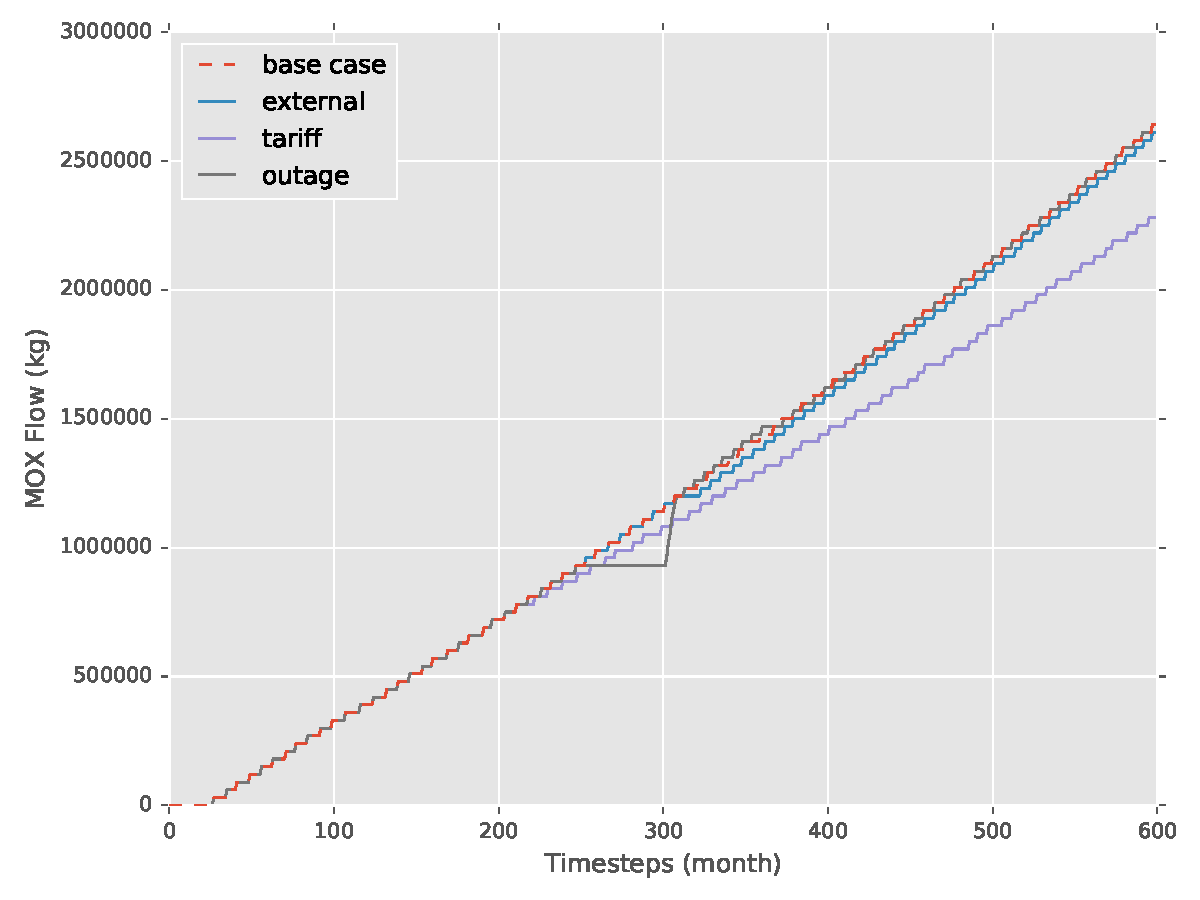
\includegraphics[width=0.9\textwidth]{mox_flow.pdf}\label{fig:moxflow}}
  \end{minipage}%
  \caption[]{
    \label{fig:flows}
    Cumulative flow of fuel in all Scenarios. The timestep period between 200
    and 400 is chosen to highlight all relevant transients. }
\end{figure}

\subsection{Solver Comparisons}

Each of the above scenarios was executed by solving the DRE using both the
\greedy heuristic and full optimization (results are shown from the \greedy
heuristic cases for clarity). Differences in simulation time are observed, as
shown in Table \ref{tbl:timing}. Solving the DRE with full optimization takes
approximately twice as long as solving it with the \greedy heuristic in these
simulations. These are small simulations and one can expect this solution time
gap to increase exponentially with simulation size, as solutions to MILPs
increase exponentially with time and the \greedy heuristic is a polynomial-time
algorithm. The primary component of simulation size that is of concern to
solution time is the total number of supply and request nodes in each
problem. These will increase with the number of entities in the simulation, the
number of commodities, and the connectedness of entities (i.e., the number of
potential transfers between entities).

\begin{table}[]
\centering
\caption{Solution times required for full simulation runs of each solver type in
  each scenario. Simulations were performed on a Macbook Air with a duel-core i5
  2.6 GHz processor using a Ubuntu 14.04 operating system.}
\label{tbl:timing}
\begin{tabular}{llr}
\toprule
Scenario & Solver & Time (s)           \\
\midrule
\basecase & cbc &     6.306 \\
          & greedy &     4.169 \\
\external & cbc &     6.371 \\
          & greedy &     3.149 \\
\outage & cbc &     5.978 \\
          & greedy &     3.161 \\
\tariff & cbc &     6.074 \\
          & greedy &     3.079 \\
\bottomrule
\end{tabular}
\end{table}

Each of the results in Table \ref{tbl:timing} is with respect to the simple
scenarios presented in this paper. In order to ascertain a sense of how each
solver will work with larger scenarios, the \basecase scenario was run an
additional time after modifying the reactor deployment schedule as follows: in
each instance when a single reactor would be deployed, five reactors are
deployed instead, increasing the total reactor population by a factor for five
to approximately 150. The greedy and cbc \basecase scenarios solved in 10.7 and
20.8 seconds, respectively. This implies that there is not a clear linear
relationship between solution time of a full simulation run and the number of
entities in the simulation for either solver -- there are likely additional
simulation dynamics occurring outside of the DRE that affect solution
times. Additionally, this simple exercise shows that simulations of reactor
populations approximately the size of the United States reactor fleet can be
solved in very reasonable times.

Interestingly, slight differences in simulation results was also observed
between the two solvers. This is due to time-steps in which there is problem
degeneracy, i.e., where multiple optimal solutions exist. Consider a timestep,
$t_i$, in which one reactor is refueling and another reactor is entering the
simulation. Four total quantities of fuel are requested - one refueling batch
and three initial core batches. Consider further that one batch of MOX fuel is
available. Because reactors all make requests to the DRE with identical
preferences, there are four degenerate optimal solutions -- one for each
potential assignment of the MOX batch. This leads to three potential simulation
futures, one in which the MOX batch is ejected after one cycle (if it assigned
to the refueling reactor or to the initial spot of the new reactor), one in
which the MOX batch is ejected after two cycles, and a third after three
cycles. In each simulation future, the quantity of fuel in the recycle loop at
$t > t_i$ is different, causing differing future behavior and overall simulation
results.
